\documentclass[border=3pt]{standalone}
\usepackage{tikz}
\usetikzlibrary{arrows.meta,calc}
\tikzset{pin/.style={-{Stealth[length=5pt]}}}
\begin{document}
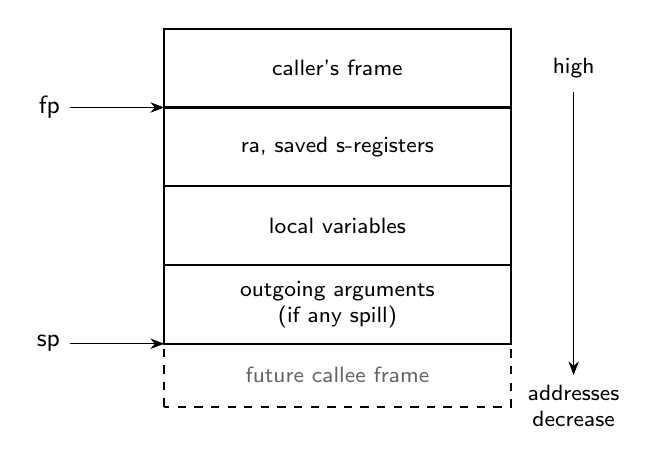
\begin{tikzpicture}[font=\sffamily\small, x=1mm, y=1mm]
  % cells top (high addresses) to bottom (low)
  \foreach \y/\h/\l in {50/10/{caller's frame}, 40/10/{ra, saved s-registers}, 30/10/{local variables}, 20/10/{outgoing arguments\\(if any spill)}}{
    \draw[thick] (0,\y) rectangle (44,\y+\h);
    \node[font=\sffamily\footnotesize, align=center] at (22,\y+\h/2) {\l};}
  \draw[thick, dashed] (0,12) rectangle (44,20);
  \node[font=\sffamily\footnotesize, text=black!60] at (22,16) {future callee frame};
  % pointers
  \draw[pin] (-12,50) node[left]{fp} -- (0,50);
  \draw[pin] (-12,20) node[left]{sp} -- (0,20);
  % address direction
  \draw[pin] (52,52) -- (52,16) node[below, font=\sffamily\footnotesize, align=center]{addresses\\decrease};
  \node[font=\sffamily\footnotesize] at (52,55) {high};
\end{tikzpicture}
\end{document}
